\chapter{Topologie-Modell für CEP-Systeme}

CEP-Systeme bilden das Grundgerüst für die Verarbeitung von Datenströmen.
Sie werden benutzt um sogenannte Topologien zu entwickeln, die von den Komponenten des CEP-Systems ausgeführt werden.
Topologien definieren über eine Abfolge von Operatoren, wie die Verarbeitung des Datenstroms stattfindet.
Die Annahmen, die über eine Topologie getroffen werden, wirken sich auf Messwerte der Topologie und den Ablauf der Verarbeitung des Datenstroms aus.
Deshalb soll in diesem Kapitel das für die vorliegende Arbeit verwendete Modell vorgestellt werden.

\section{Topologie als Graph}

In der Literatur werden Topologien oft als Graph dargestellt.
Dabei werden Operatoren als Knoten und der Fluss des Datenstroms zwischen Operatoren als Kanten dargestellt.
Das in dieser Arbeit verwendete Topologie-Modell besteht aus zwei unterschiedlichen gerichteten azyklischen Graphen.
Die Darstellung der Topologie durch zwei Graphen wurde ebenfalls von Lohrmann et al. \cite{lohrmann_elastic_2015} verwendet.
Ein Graph beschreibt den logischen Aufbau der Topologie, während der andere Graph die physische Ausdehnung der Topologie beschreibt.
Die Graphen sind dabei direkt voneinander abhängig und stellen verschiedene Sichtweisen auf die Topologie dar.
In Abbildung 4.1 ist der logische Aufbau einer Topologie dargestellt. 
Sie beschreibt die Abfolge von Operatoren, die die Tupel des Datenstroms verarbeiten.

\begin{figure}
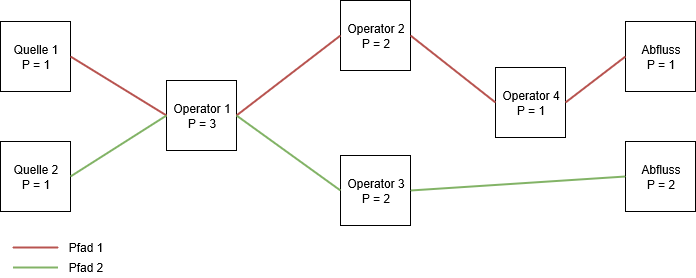
\includegraphics[scale=0.6]{LogischesModell}
\caption{Modell der logischen Topologie}
\end{figure}

In der dargestellten Topologie sind zwei Pfade beschrieben.
Ein Pfad ist durch die Verkettung der Operatoren mit der grünen Linie dargestellt.
Ein Weiterer wird durch die braune Linie beschrieben.
Das erste Element eines Pfades ist die sogenannte Quelle, eine spezielle Form des Operators.
Sie führt Tupel aus einem externen Datenstrom in die Topologie ein.
Tupel sind einzelne Elemente eines Datenstroms, z.B. ein JSON-Objekt.
Das Ende eines Pfads ist immer der Konsument.
Dieser ist der letzte Operator an denen die Tupel aus der Quelle verarbeitet werden. 
Oft werden die Tupel hier an ein anderes System weiter gegeben, in eine Datenbank geschrieben oder auch verworfen.
Die Tupel bewegen sich entlang eines Pfades.

Zwischen der Quelle und dem Abfluss befinden sich weitere Operatoren. 
Diese beinhalten Funktionen, mit denen die Tupel bearbeitet werden.
Nachdem die Funktion ausgeführt wurde, sendet der Operator das Tupel an den nächsten Operator auf dem festgelegten Pfad.
Der nächste Operator wird auch als Nachfolger bezeichnet.
Der Operator, von dem der Operator Tupel empfängt wird als Vorgänger bezeichnet.
So ist in Abbildung 4.1 Operator 1 der Vorgänger von Operator 2, der wiederum der Nachfolger von Operator 1 ist.
Ein Operator kann, wie in der Abbildung skizziert, auch auf mehreren Pfaden vorhanden sein. 
Allerdings kann ein spezifischer Operator nur einmal innerhalb eines Pfades auftreten, da es sich um einen azyklischen Graph handelt.

In der gezeigten Topologie wird davon ausgegangen, dass Tupel selektiv weitergeleitet werden können.
Das bedeutet, dass ein Operator, welcher sich auf mindestens zwei Pfaden befindet, die Tupel nicht an alle Nachfolger sendet.
Er selektiert stattdessen welche Tupel er an welchen Nachfolger sendet.
Wie in der Abbildung 4.1 dargestellt sendet Operator 1 die Tupel von Quelle 2 nur an Operator 3 weiter.
Die Tupel von Quelle 1 werden nur an Operator 2 weitergeleitet.
Würden die Tupel jeweils an beide Folgeoperatoren (Operator 2 und Operator 3) weitergeleitet werden, würde die Topologie vier Pfade aufweisen.
Dann beschreibt ein Pfad den Weg von Quelle 1 zu Konsument 2 und der vierte Pfad von Quelle 2 zu Konsument 1.

Alle Operatoren besitzen einen Parallelisierungsgrad.
Dieser bestimmt den Aufbau des zweiten Graphen. 
Der Parallelisierungsgrad ist mindestens eins und kann einen beliebigen aber fixierten Maximalwert nicht überschreiten. 
Die Quelle besitzt laut diesem Modell zwar einen Parallelisierungsgrad, wird jedoch von den nachfolgend implementierten Algorithmen, die die Topologie skalieren, nicht berücksichtigt.
Die Quelle wird in vielen Arbeiten als nicht parallelisierbar modelliert und wird deshalb von vielen Algorithmen nicht betrachtet.

\begin{figure}
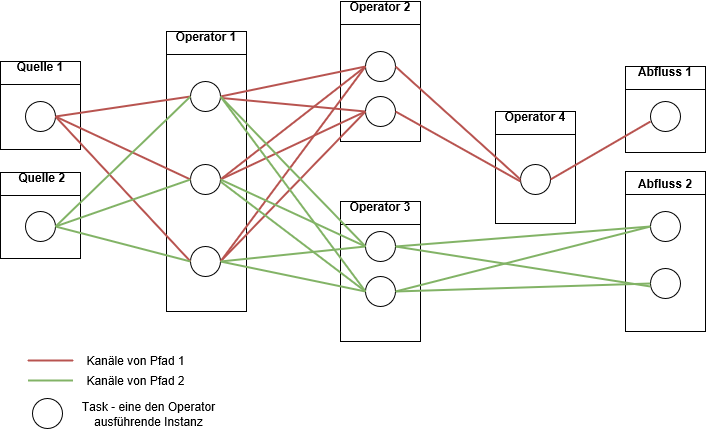
\includegraphics[scale=0.6]{PhysischesModell}
\caption{Modell der physischen Topologie}
\end{figure}

Abbildung 4.2 zeigt die beiden Pfade in der Form, wie sie im CEP-System physisch ausgeprägt sind.
Dies entspricht dem zweiten Graph im vorgestellten Topologie-Modell.
Jeder Operator besitzt genau die Anzahl Tasks, die durch den Parallelisierungsgrad festgelegt ist.
Ein Task ist eine Instanz, welche die Funktion des logischen Operators ausführt.
Zwischen den Tasks befinden sich Kanäle, über die diese miteinander kommunizieren.
Ein Task hat dabei immer einen Kanal zu allen Tasks des folgenden Operators.
So kann ein Tupel von diesem zu jedem beliebigen Task des Nachfolgers gesendet werden.
Die Tasks der Topologie können auf verschiedenen Rechnern verteilt sein und über ein Netzwerk kommunizieren.
Das Modell geht dabei davon aus, das allen Tasks die gleiche Größe von Rechenleistung und Speicher für die Ausführung der Operation zur Verfügung stehen.
Da Quelle und Konsument jeweils die Enden der Topologie darstellen, gibt es keine eingehenden Kanäle an der Quelle sowie keine ausgehenden Kanäle an dem Konsumenten.

Wird ein Tupel an den Nachfolger gesendet, so wird es immer nur an einen einzigen Task des Nachfolgers verschickt.
Für die Vorgehensweise wie der Task des Nachfolgers ausgewählt gibt es verschiedene Ansätze.
Dies kann zum einen per Zufall geschehen.
Eine andere Möglichkeit ist die Zuordnung zu einem bestimmten Task über ein Feld des Tupels.
Eine weitere Möglichkeit ist das Weiterleiten zu einem speziellen Task über einen bestimmten Zeitraum.
Die letzten beiden Methoden sind sinnvoll, wenn der Folgeoperator eine Funkion implementiert die ein Fenster verwendet.
Für die Lösung, welcher Task des Nachfolgers das Tupel verarbeitet, gibt es, wie in Kapitel 2 und 3 beschrieben, eine Auswahl dedizierter Algorithmen.
Die Entscheidung, wie die Tupel zwischen Tasks weitergeleitet werden, hat keinen Einfluss auf die selektive Weiterleitung, die zwischen Operatoren auf logischer Ebene definiert ist.

\section{Messwerte}

Um den Datenfluss durch die Topologie zu überwachen, werden Messwerte erfasst.
Diese dienen der Analyse der Topologie als Ganzes und der Untersuchung einzelner Operatoren.
Wenn ein Operator eines Pfads sehr langsam arbeitet, bremst er alle Tupel des gesamten Pfads.
Mit Hilfe der Messwerte können solche Engpässe identifiziert und durch Skalieren des Operators behoben werden.
Die in Kapitel 3 vorgestellten Algorithmen berechnen mit Hilfe der Messwerte den neuen Parallelisierungrad eines Operators.

Das Modell geht davon aus, dass die gemessenen Werte eines Operators unabhängig von dessen Pfad sind.
Dies bedeutet, dass ein Operator, der auf zwei oder mehr verschiedenen Pfaden liegt, bei den Messwerten nicht zwischen den Pfaden unterscheidet.
Diese Annahme erfordert, dass Tupel unabhängig davon über welchen Pfad sie beim Operator ankommen den gleichen Aufwand erzeugen.
Sind die Messwerte für die Tasks eines Operators bekannt, kann der Messwert für den Operator aus den Messwerten der Tasks aggregiert werden.
Zähler werden dabei summiert, für die anderen Messwerte der Durchschnitt ermittelt.
Für das Modell werden folgenden Messwerte definiert.
Die Messwerte, die für Tasks beschrieben sind, gelten unter der Annahme, dass sie aggregiert wurden, ebenso für Operatoren.

\begin{itemize}
\item{Pfad-Latenz / Tupel-Latenz: Beschreibt die durchschnittliche Dauer in Millisekunden, die ein Tupel benötigt um die Topologie von der Quelle bis zum Konsumenten zu durchqueren. 
Die Dauer beginnt mit der Abgabe des Tupels durch die Quelle bis es vom Konsumenten erfolgreich abgearbeitet wurde. 
Die Messung ist nur zuverlässig, wenn Quelle und Konsument auf dem gleichen Rechner platziert sind, da Uhren verschiedener Rechner nicht zu 100\% synchron sind \cite{goggel_vergleich_20180}.}
\item{Fehlgeschlagene Tupel: Gibt die Anzahl Tupel an,  bei denen die Verarbeitung in der Topologie nicht erfolgreich war.
Ursache kann unter anderem ein Fehler während der Bearbeitung durch einen Operator sein.}
\item{Bestätigte Tupel: Anzahl der Tupel, die erfolgreich durch die Topologie abgearbeitet wurden.}
\item{Task-Latenz: Die durchschnittliche Dauer in Millisekunden, die ein Task benötigt um ein Tupel wieder abzugeben. 
Diese unterscheidet sich bei Operatoren die ein Fenster verwenden und Operatoren die kein Fenster verwenden  \cite{lohrmann_elastic_2015}.
Ein Fenster beschreibt einen Operators der Tupel aufnimmt, um auf allen gesammelten Tupeln eine Operation durchzuführen.
Meistens erfordert die Operation mehrere Tupel um Zusammenhänge zu erkennen.
Die Latenz des ersten aufgenommenen Tupels ist dann länger als die des Tupels welches zuletzt in das Fenster aufgenommen wurde, da sie alle zusammen wieder weitergeleitet werden wenn das Fenster voll ist. 
Verwendet der Operator kein Fenster, so wird das Tupel direkt nach der Aufnahme verarbeitet und weitergeleitet.
Anschließend wird das nächste Tupel aufgenommen.}
\item{Anzahl Ausführungen des Tasks: Misst die Anzahl wie oft der Task ein neues Tupel aufgenommen und verarbeitet hat.}
\item{Anzahl eingehender Tupel: Misst die Anzahl der Tupel, die beim Task ankommen. Der Messwert ist nicht identisch mit der Anzahl Ausführungen des Tasks, da sich vor dem Task ein Buffer befindet, in dem Tupel zwischengespeichert werden können bevor sie verarbeitet werden.}
\item{Anzahl ausgehender Tupel: Misst die Anzahl der Tupel, die vom Task versendet wurden. Tupel die auf mehreren Pfaden ausgeben werden, werden nicht mehrfach gezählt.}
\item{Bearbeitungsdauer: Beschreibt die durchschnittliche Dauer in Millisekunden, die zwischen der Aufnahme von Tupeln zur Bearbeitung liegt. 
Die Bearbeitungsdauer ist für Operatoren ohne Fenster gleich der Latenz \cite{lohrmann_elastic_2015}.}
\item{Tupel-Ankunftsintervall: Beschreibt die durchschnittliche Dauer in Millisekunden, die zwischen der Ankunft von zwei Tupeln am Task vergeht.}
\item{Auslastung: Gibt die Auslastung des Tasks in Prozent an. Die Auslastung kann unter anderem durch \(\frac{Bearbeitungsdauer}{Tupel-Ankunftsintervall}\) berechnet werden.}
\item{Varianz der Bearbeitungsdauer: Gibt die Varianz der Stichprobe von Messwerten der Bearbeitungsdauer an.}
\item{Varianz des Tupel-Ankunftsintervalls: Gibt die Varianz der Stichprobe von Messwerten des Tupel-Ankunftsintervalls an.}
\item{Latenz des Kanals: Gibt die durchschnittliche Latenz eines Kanals zwischen zwei Tasks in Millisekunden an. 
Die Dauer beginnt ab der Ausgabe des Tupels durch den Vorgänger-Task bis zur Aufnahme des Tupel durch den Nachfolge-Task.
Die Latenz des Kanals beinhaltet insbesondere die Zeit im Ausgangs-Zwischenspeicher des Vorgänger-Task, die Netzwerklatenz und die Zeit im Eingangs-Zwischenspeicher des Nachfolge-Task.}
\item{Latenz der Stapelverarbeitung: Die durchschnittliche Dauer in Millisekunden, die ein Tupel im Ausgangs-Zwischenspeicher des Vorgänger-Task liegt.}
\end{itemize}